%!TEX root = ../dissertation.tex
\begin{savequote}[75mm]
Nulla facilisi. In vel sem. Morbi id urna in diam dignissim feugiat. Proin molestie tortor eu velit. Aliquam erat volutpat. Nullam ultrices, diam tempus vulputate egestas, eros pede varius leo.
\qauthor{Quoteauthor Lastname}
\end{savequote}

\chapter{The title of chapter one}

\newthought{There's something to be said} Fermat's Little Theorem states that for any integer $a$ and any prime number $p$, the following congruence relation holds:

\begin{equation}
    a^p\equiv a\mod p
\end{equation}

An example of a figure is shown in Figure \ref{fig:fig1}.

\begin{figure}[H]\centering
    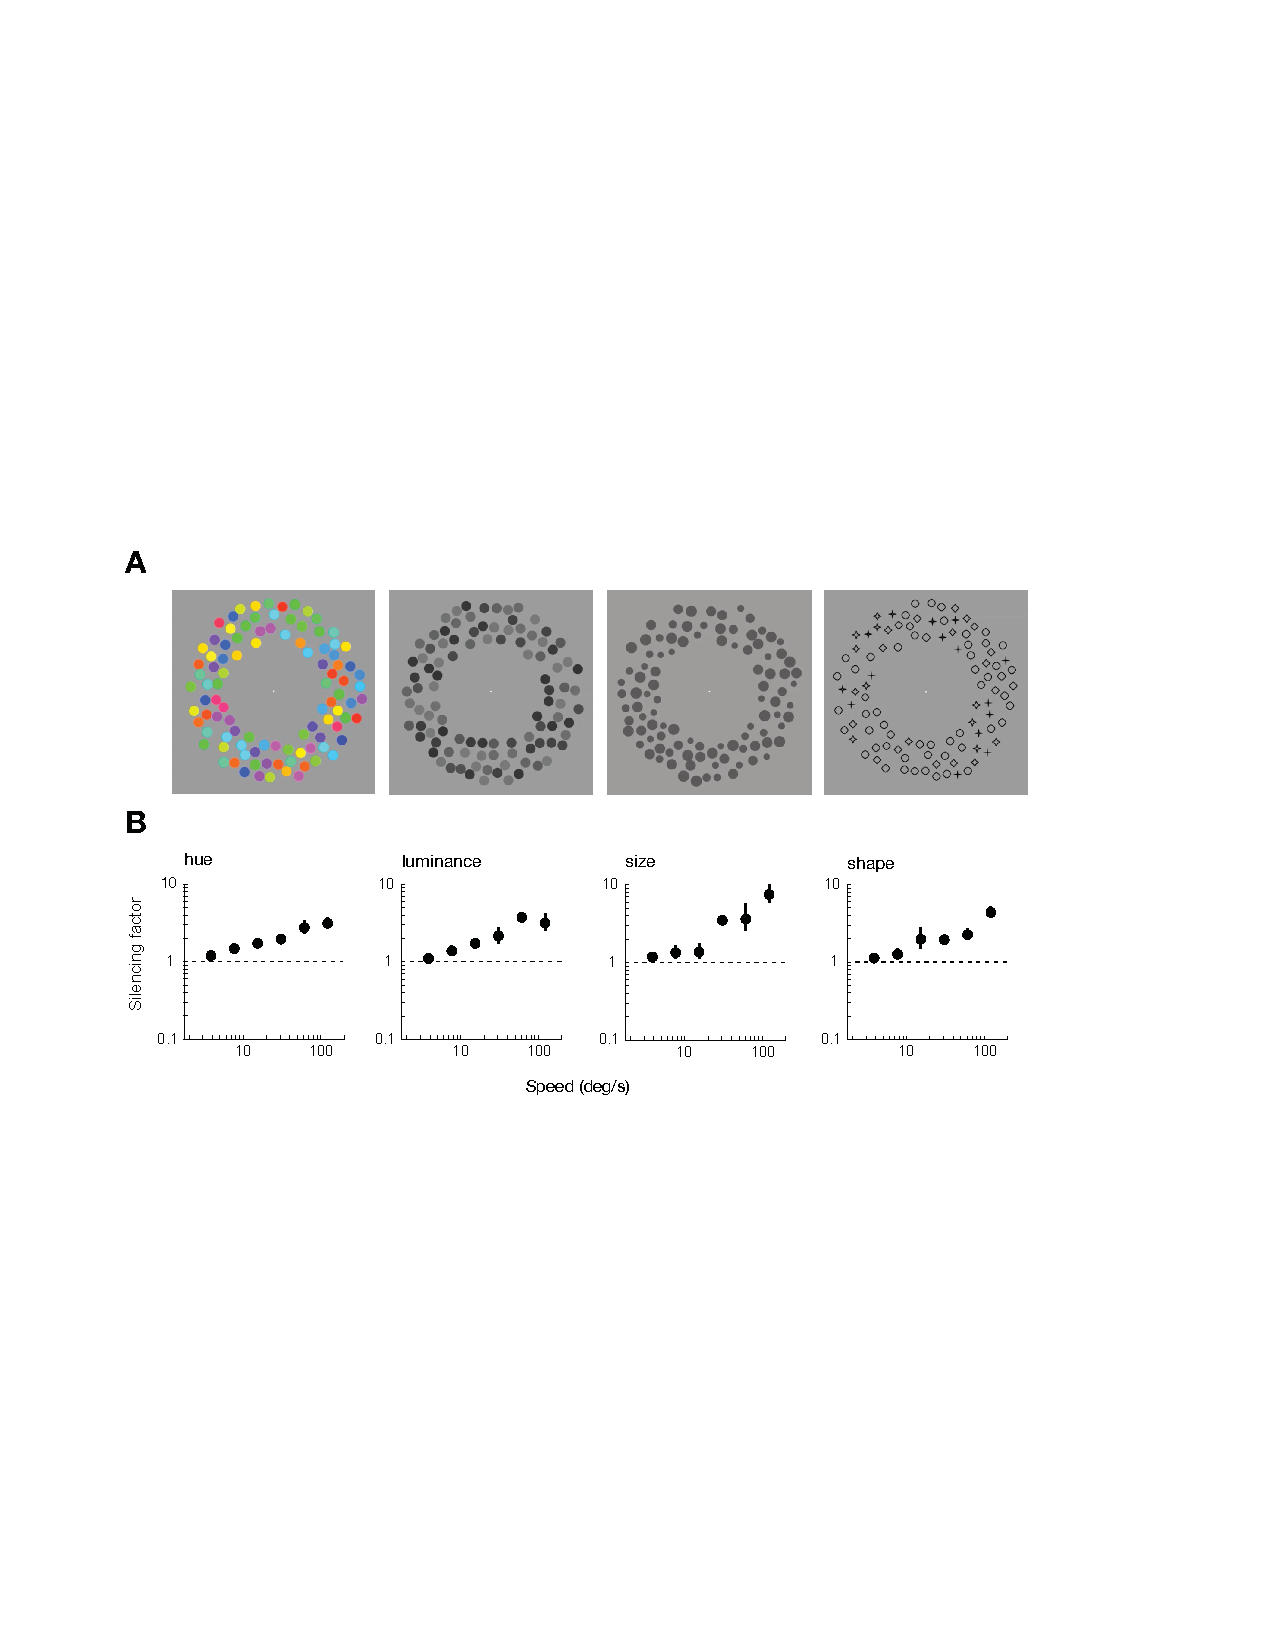
\includegraphics[width=\textwidth]{figures/fig1.pdf}
    \caption[
        Figure 1
    ]{
        Figure 1
    }\label{fig:fig1}
\end{figure}


An example of a table is shown in Table \ref{tab:tab1}.

\begin{table}[H]\centering\caption{
    Table 1
}\label{tab:tab1}
	\begin{tabular}{cccc}\hline
        Col1 & Col2 & Col3 & Col4\\\hline
        1 & 2 & 3 & 4\\
        5 & 6 & 7 & 8\\
        9 & 10 & 11 & 12\\
		\hline
	\end{tabular}
\end{table}